% F049: native TikZ/PGFPlots, computed from the stated mathematical model.
\begin{center}
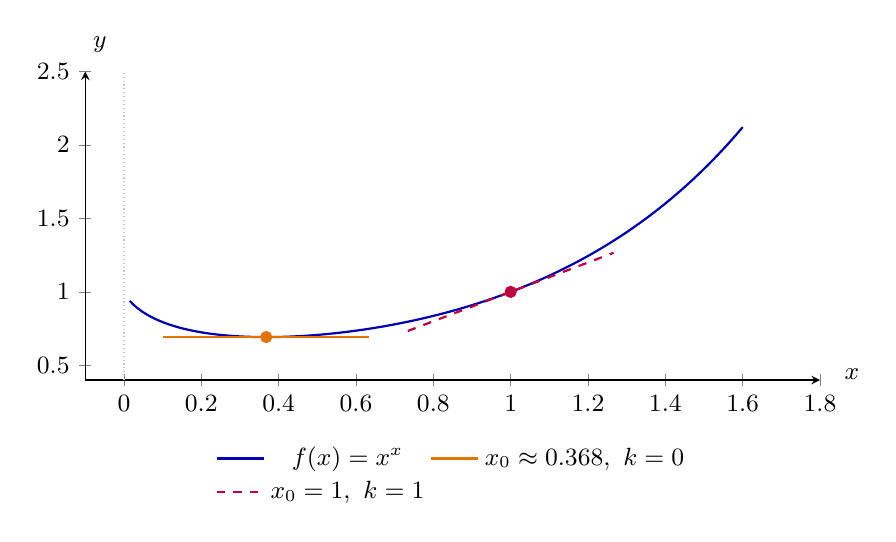
\begin{tikzpicture}[font=\small,>=stealth]
\begin{axis}[width=.90\linewidth,height=5.5cm,xmin=-0.1,xmax=1.8,ymin=0.4,ymax=2.5,
axis lines=left,xlabel={$x$},ylabel={$y$},font=\small,
xlabel style={at={(axis description cs:1.02,.02)},anchor=west},
ylabel style={rotate=-90,at={(axis description cs:.02,1.03)},anchor=south},
legend style={at={(axis description cs:.5,-.18)},anchor=north,draw=none,fill=none,font=\small,legend columns=2},
unbounded coords=jump,clip=true,]
\addplot[gray!45,thin,densely dotted,forget plot] coordinates {(0,0.4) (0,2.5)};
\addplot[blue!70!black,thick] coordinates {(0.015,0.93894763) (0.023805556,0.91486271) (0.032611111,0.89437407) (0.041416667,0.87645173) (0.050222222,0.86051037) (0.059027778,0.84617111) (0.067833333,0.8331686) (0.076638889,0.82130681) (0.085444444,0.81043524) (0.09425,0.8004349) (0.10305556,0.79120956) (0.11186111,0.78267992) (0.12066667,0.77477965) (0.12947222,0.76745255) (0.13827778,0.76065049) (0.14708333,0.75433187) (0.15588889,0.74846044) (0.16469444,0.74300438) (0.1735,0.7379356) (0.18230556,0.73322914) (0.19111111,0.72886275) (0.19991667,0.72481649) (0.20872222,0.72107239) (0.21752778,0.71761424) (0.22633333,0.71442737) (0.23513889,0.71149841) (0.24394444,0.70881521) (0.25275,0.70636666) (0.26155556,0.70414259) (0.27036111,0.70213368) (0.27916667,0.70033137) (0.28797222,0.69872775) (0.29677778,0.69731556) (0.30558333,0.6960881) (0.31438889,0.69503915) (0.32319444,0.69416299) (0.332,0.6934543) (0.34080556,0.69290816) (0.34961111,0.69252001) (0.35841667,0.69228561) (0.36722222,0.69220103) (0.37602778,0.69226264) (0.38483333,0.69246704) (0.39363889,0.69281108) (0.40244444,0.69329186) (0.41125,0.69390666) (0.42005556,0.69465298) (0.42886111,0.69552848) (0.43766667,0.69653101) (0.44647222,0.69765859) (0.45527778,0.69890937) (0.46408333,0.70028165) (0.47288889,0.70177388) (0.48169444,0.70338461) (0.4905,0.70511253) (0.49930556,0.70695646) (0.50811111,0.70891529) (0.51691667,0.71098804) (0.52572222,0.71317383) (0.53452778,0.71547186) (0.54333333,0.71788143) (0.55213889,0.72040191) (0.56094444,0.72303278) (0.56975,0.72577357) (0.57855556,0.72862391) (0.58736111,0.73158349) (0.59616667,0.73465207) (0.60497222,0.73782948) (0.61377778,0.74111561) (0.62258333,0.74451043) (0.63138889,0.74801396) (0.64019444,0.75162628) (0.649,0.75534752) (0.65780556,0.75917789) (0.66661111,0.76311762) (0.67541667,0.76716704) (0.68422222,0.77132649) (0.69302778,0.77559638) (0.70183333,0.77997717) (0.71063889,0.78446937) (0.71944444,0.78907353) (0.72825,0.79379027) (0.73705556,0.79862022) (0.74586111,0.8035641) (0.75466667,0.80862265) (0.76347222,0.81379664) (0.77227778,0.81908693) (0.78108333,0.82449439) (0.78988889,0.83001994) (0.79869444,0.83566455) (0.8075,0.84142923) (0.81630556,0.84731503) (0.82511111,0.85332306) (0.83391667,0.85945445) (0.84272222,0.86571039) (0.85152778,0.87209211) (0.86033333,0.87860087) (0.86913889,0.88523798) (0.87794444,0.89200481) (0.88675,0.89890276) (0.89555556,0.90593325) (0.90436111,0.91309779) (0.91316667,0.9203979) (0.92197222,0.92783516) (0.93077778,0.93541118) (0.93958333,0.94312762) (0.94838889,0.95098619) (0.95719444,0.95898865) (0.966,0.96713679) (0.97480556,0.97543245) (0.98361111,0.98387753) (0.99241667,0.99247396) (1.0012222,1.0012237) (1.0100278,1.0101288) (1.0188333,1.0191914) (1.0276389,1.0284135) (1.0364444,1.0377974) (1.04525,1.0473453) (1.0540556,1.0570594) (1.0628611,1.0669421) (1.0716667,1.0769958) (1.0804722,1.0872228) (1.0892778,1.0976258) (1.0980833,1.1082071) (1.1068889,1.1189695) (1.1156944,1.1299156) (1.1245,1.141048) (1.1333056,1.1523696) (1.1421111,1.1638831) (1.1509167,1.1755914) (1.1597222,1.1874976) (1.1685278,1.1996045) (1.1773333,1.2119153) (1.1861389,1.2244331) (1.1949444,1.237161) (1.20375,1.2501023) (1.2125556,1.2632604) (1.2213611,1.2766387) (1.2301667,1.2902405) (1.2389722,1.3040694) (1.2477778,1.318129) (1.2565833,1.332423) (1.2653889,1.3469551) (1.2741944,1.3617292) (1.283,1.3767491) (1.2918056,1.3920188) (1.3006111,1.4075423) (1.3094167,1.4233238) (1.3182222,1.4393674) (1.3270278,1.4556776) (1.3358333,1.4722585) (1.3446389,1.4891148) (1.3534444,1.5062509) (1.36225,1.5236715) (1.3710556,1.5413813) (1.3798611,1.5593852) (1.3886667,1.5776879) (1.3974722,1.5962947) (1.4062778,1.6152105) (1.4150833,1.6344405) (1.4238889,1.6539901) (1.4326944,1.6738647) (1.4415,1.6940699) (1.4503056,1.7146111) (1.4591111,1.7354942) (1.4679167,1.7567249) (1.4767222,1.7783094) (1.4855278,1.8002535) (1.4943333,1.8225636) (1.5031389,1.8452459) (1.5119444,1.8683069) (1.52075,1.891753) (1.5295556,1.9155911) (1.5383611,1.9398279) (1.5471667,1.9644704) (1.5559722,1.9895256) (1.5647778,2.0150008) (1.5735833,2.0409033) (1.5823889,2.0672406) (1.5911944,2.0940205) (1.6,2.1212506)};
\addlegendentry{$f(x)=x^x$}
\addplot[orange!90!black,thick] coordinates {(0.10187944,0.69220063) (0.63387944,0.69220063)};
\addlegendentry{$x_0\approx0.368,\ k=0$}
\addplot[only marks,mark=*,orange!90!black,forget plot] coordinates {(0.36787944,0.69220063)};
\addplot[purple,thick,dashed] coordinates {(0.734,0.734) (1.266,1.266)};
\addlegendentry{$x_0=1,\ k=1$}
\addplot[only marks,mark=*,purple,forget plot] coordinates {(1,1)};

\end{axis}
\end{tikzpicture}
\par\smallskip{\small $x>0$；在 $x=1/e$ 处由下降转为上升。}
\end{center}
